\documentclass[11pt]{article}
\usepackage[utf8]{inputenc}

\usepackage[table,xcdraw]{xcolor}
\usepackage{graphicx}
\usepackage[english]{babel}
\usepackage[framemethod=default]{mdframed}
\usepackage{tocloft}
\usepackage{adjustbox}
\usepackage{todonotes}
\usepackage{float}
\usepackage{pbox}
\usepackage{enumitem}
\usepackage{comment}
\usepackage{makecell}
\usepackage{lipsum}
\usepackage{caption}
\usepackage{hyperref}
\usepackage{subcaption}
\usepackage[linesnumbered,ruled,vlined]{algorithm2e}
\usepackage{fancyhdr}

\newcommand\Tstrut{\rule{0pt}{2.6ex}}       % "top" strut
\newcommand\Bstrut{\rule[-0.9ex]{0pt}{0pt}} % "bottom" strut
\newcommand{\TBstrut}{\Tstrut\Bstrut} % top&bottom struts

%----------------------------------------------------------------------------------------
%	TITLE PAGE
%----------------------------------------------------------------------------------------

\newcommand*{\titleGM}{\begingroup % Create the command for including the title page in the document

\hbox{ % Horizontal box
\hspace*{0.03\textwidth} % Whitespace to the left of the title page
\rule{1pt}{\textheight} % Vertical line
\hspace*{0.05\textwidth} % Whitespace between the vertical line and title page text
\parbox[b]{0.75\textwidth}{ % Paragraph box which restricts text to less than the width of the page

{\noindent\Huge\bfseries Computer \\[0.2\baselineskip] Vision \large(H02A5A)}\\[2\baselineskip] % Title
{\huge Project report}\\[2\baselineskip] % Title
{\large \textit{Incisor Segmentation}}\\[4\baselineskip] % Tagline or further 
{\Large \textsc{Kristof Arron - r0467804}}\\[0.2\baselineskip]
{\Large \textsc{Robin Haveneers - r0450702}}\\[4\baselineskip]
\small \textsc{Prof. dr. ir. Dirk Vandermeulen}\\
\small \textsc{2016-2017}

\vspace{0.25\textheight}
% Whitespace between the title block and the publisher
{\noindent 
\includegraphics[scale=0.5]{kul-color.jpg}}\\[\baselineskip] % Publisher and logo
}}
\endgroup}

\begin{document}

\begin{titlepage}
\pagestyle{empty}
\titleGM % This command includes the title page
\end{titlepage}

\pagestyle{fancy} % Turn on the style
\fancyhf{} % Start with clearing everything in the header and footer
% Set the right side of the footer to be the page number
\renewcommand{\headrulewidth}{0pt}
\fancyfoot[R]{\thepage}

% Redefine plain style, which is used for titlepage and chapter beginnings
% From https://tex.stackexchange.com/a/30230/828
\fancypagestyle{plain}{%
    \renewcommand{\headrulewidth}{0pt}%
    \fancyhf{}%
    \fancyfoot[R]{\thepage}%
}

\tableofcontents

\newpage

\section{Introduction}

This report describes the process of both the manual and automatic segmentation of all eight incisor teeth in different dental panoramic radiographs. We use the Active Shape Model (ASM) method to segment the teeth. First we discuss how to build such a model. We briefly mention the steps that are needed to process the data before a model can be built. Next we analyse the results of ASM via Principal Component Analysis (PCA). This gives us an illustration of the most important modes of variation within the shape of each tooth. A next section describes the preprocessing steps that are taken on the radiographs in order to reduce noise and improve contrast. Thereafter we explain how to fit the model to new images, either manually or automated. We end the report with a short evaluation of the results and a brief discussion on the project.

\newpage

\section{Building an Active Shape Model}
\subsection{Generalized Procrustes Analysis}
In this first part of building the Active Shape Model, it is important that the given landmarks are represented in the same coordinate frame. The shape of the landmarks should be independent of the position, scale and orientation of the tooth. This is where we applied the Procrustes Analysis. As described in \cite{cootes2000introduction}, we align the set of training shapes into a common frame. The goal is to align each shape such that the sum of distances of each shape to the mean shape is minimised.
\newline~\newline
Below, on the left hand side in figure \ref{fig:unaligned} you can see a plot of all the landmarks of the first incisor. On the right hand side, in figure \ref{fig:aligned}, you can see the same shapes, centered around the origin, having a mean scale of unity and having a fixed but arbitrary orientation.

\begin{figure}[H]
\centering
\begin{minipage}{.5\textwidth}
  \centering
  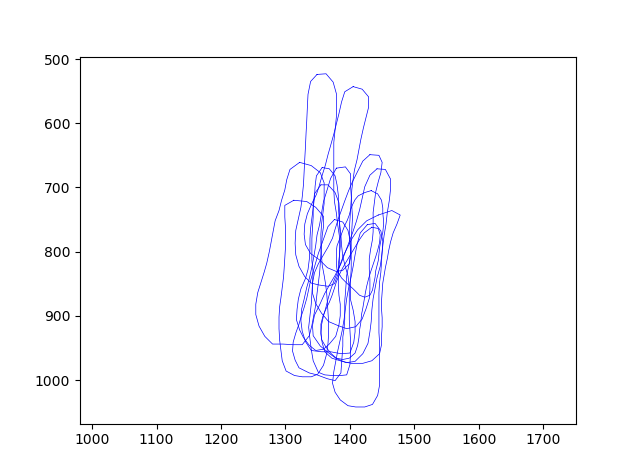
\includegraphics[width=\linewidth]{unaligned_shapes}
  \captionof{figure}{Unaligned shapes\\ of tooth 1}
  \label{fig:unaligned}
\end{minipage}%
\begin{minipage}{.5\textwidth}
  \centering
  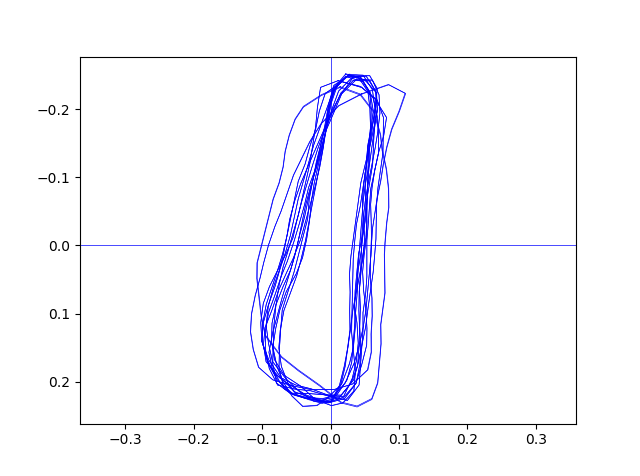
\includegraphics[width=\linewidth]{aligned_shapes}
  \captionof{figure}{Aligned shapes\\ of tooth 1}
  \label{fig:aligned}
\end{minipage}
\end{figure}


\subsection{Principal Component Analysis}
Once all shapes are aligned, we can perform Principal Component Analysis on these new shapes. The result of this analysis is a set of principal components or modes of variation. These modes describe the directions with the largest variance within the data. Figure \ref{fig:modes} shows the three most important principal components and the shape variations they allow. PCA allows us to reduce the dimensionality of the dataset by keeping only a subset of the principal components, while still explaining a high percentage of the variance. In this application, the amount of modes needed to explain over 99\% of the variance is determined dynamically for each tooth. However, usually about 7 to 9 modes are needed, table \ref{tbl:variance} shows this for tooth 1 and 8, other teeth are similar.  

\begin{figure}[H]
  \centering
  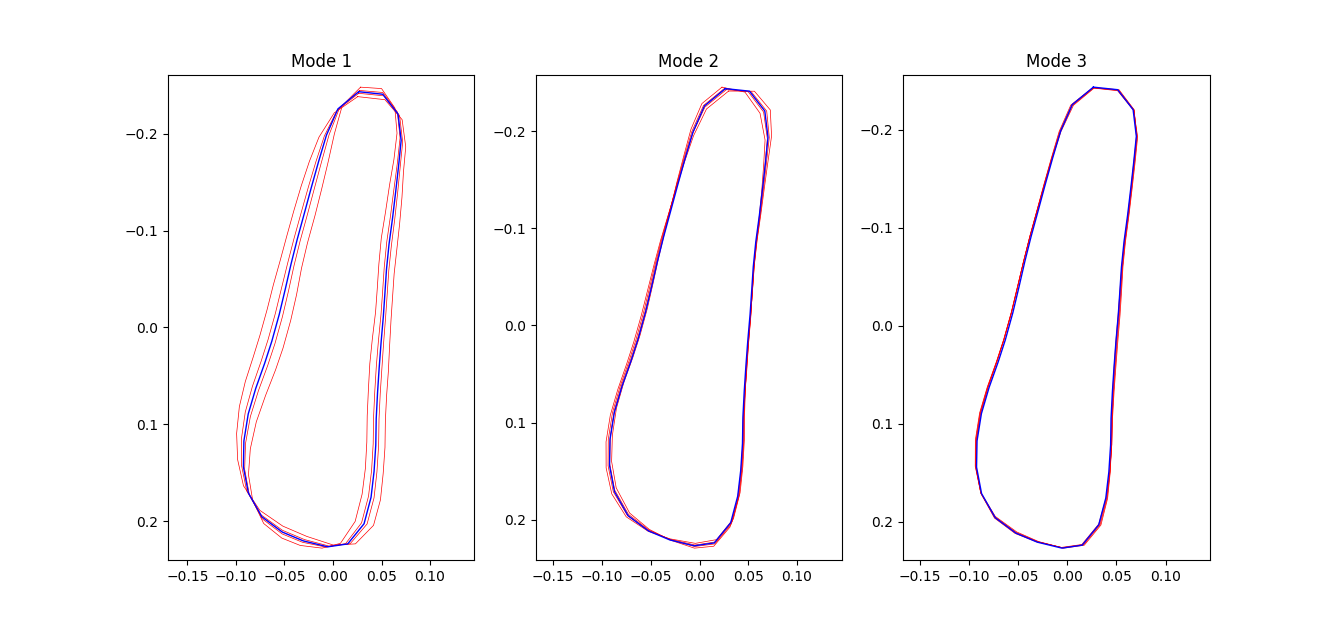
\includegraphics[width=\linewidth]{modes_and_mean}
  \captionof{figure}{Variation of the 3 most important principal components. The blue shape is the mean shape, the red shapes indicate possible variations.}
  \label{fig:modes}
\end{figure}

\begin{table}[H]
\centering
\begin{tabular}{c|c|c}
						& \textbf{Tooth 1} & \textbf{Tooth 8}  \TBstrut      \\ \hline
\multicolumn{1}{l|}{1} & 0.646400530498 & 0.42062844717 \TBstrut \\ \hline
\multicolumn{1}{l|}{2} & 0.898917160953 & 0.752692890297 \TBstrut\\ \hline
\multicolumn{1}{l|}{3} & 0.949902073345 & 0.868618769304 \TBstrut\\ \hline
\multicolumn{1}{l|}{4} & 0.971813974816 & 0.927944903926 \TBstrut\\ \hline
\multicolumn{1}{l|}{5} & 0.980536831643 & 0.957612924558 \TBstrut\\ \hline
\multicolumn{1}{l|}{6} & 0.98736569597  & 0.972696635066 \TBstrut\\ \hline
\multicolumn{1}{l|}{7} & 0.991154402009 & 0.981115590281 \TBstrut\\ \hline
\multicolumn{1}{l|}{8} &                & 0.987446059787 \TBstrut\\ \cline{1-1} \cline{3-3}
\multicolumn{1}{l|}{9} &                & 0.992000005508 \TBstrut\\ 
\end{tabular}
\caption{Examples of the amount of principal components needed to reach 99\% variance.}
\label{tbl:variance}
\end{table}

\section{Preprocessing the Radiographs}

Radiographs are prone to noise. In order to use the images for detection, we need to reduce the noise. In our application, we apply different filters to the images according to tactics described in \cite{imageenhance} and \cite{imageenhance2}. All images are first filtered with a Gaussian filter of size 3. This reduces noise but also blurs the image, making edges less distinct. The second filter is a median filter of size 7. This filter aims to reduce noise while keeping edges clear. The next filter is a hatfilter. This is composed of two separate filters. A white hat and a black hat filter. The black hat filter enhances dark features, while the white hat filter enhances bright features. The last filter that is applied to the radiographs is an adaptive histogram equalisation filter. This filter increases contrast.

~\\
The result of applying these filters is an image that is more suitable for edge detection. This is advantageous since we primarily use the strongest edge method to fit the tooth model to the images. The last step in the process is to detect the edges with the Sobel operators. Examples of the results of each step of the filtering process can be seen in figures \ref{fig:hat}, \ref{fig:ahe} and \ref{fig:sobel}. The median and Gaussian filter steps are not included.

\begin{figure}[H]
\centering
\begin{minipage}{.30\textwidth}
  \centering
  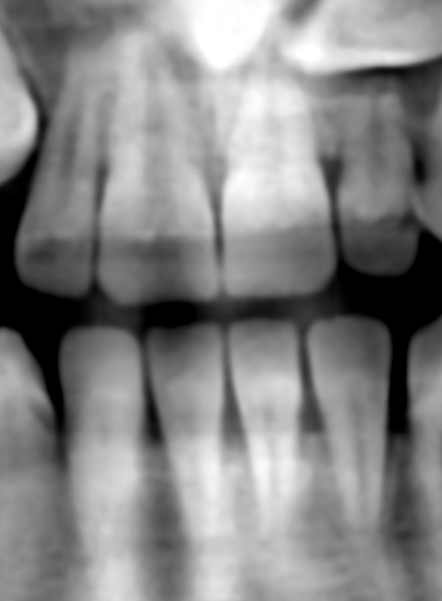
\includegraphics[width=\linewidth]{HATcropped}
  \captionsetup{justification=centering}
  \captionof{figure}{Result of hatfilter}
  \label{fig:hat}
\end{minipage}%
\hspace{1em}
\begin{minipage}{.30\textwidth}
  \centering
  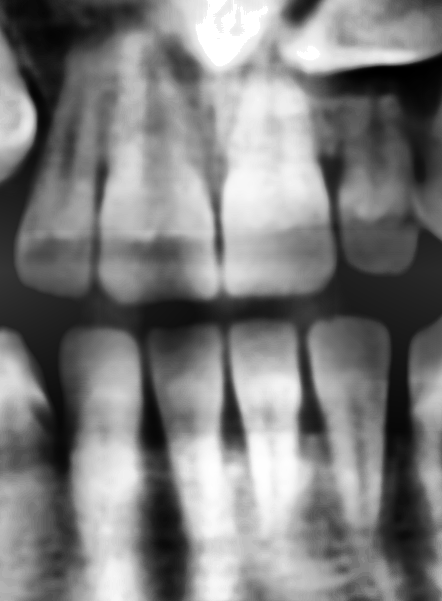
\includegraphics[width=\linewidth]{AHEcropped}
  \captionsetup{justification=centering}
  \captionof{figure}{Result of AHE filter}
  \label{fig:ahe}
\end{minipage}%
\hspace{1em}
\begin{minipage}{.30\textwidth}
  \centering
  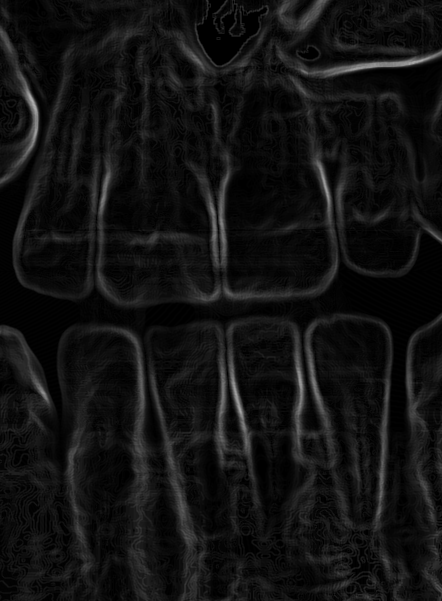
\includegraphics[width=\linewidth]{SOBELcropped}
  \captionsetup{justification=centering}
  \captionof{figure}{Result of Sobel detector}
  \label{fig:sobel}
\end{minipage}
\end{figure}

\section{Fitting the Model to Images}
Fitting the found model to the images starts by finding an initial estimate for the model in the image. We developed a manual and an automatic initialization method, as described below. Next, the model is fitted to the image in an iterative manner. Our approach is primarily based on the methods described in \cite{cootes2000introduction} and \cite{cootestraining}.

\subsection{Manual Initialization}
In the manual initialization, the user is presented with the radiograph of the person for whom he is trying to fit the model, as can be seen in figure \ref{fig:manual}. He can use his mouse to drag the shape to the correct incisor and when a key is pressed, the current selection is used. The selection defines 40 initial landmark coordinates.
\begin{figure}[H]
  \centering
  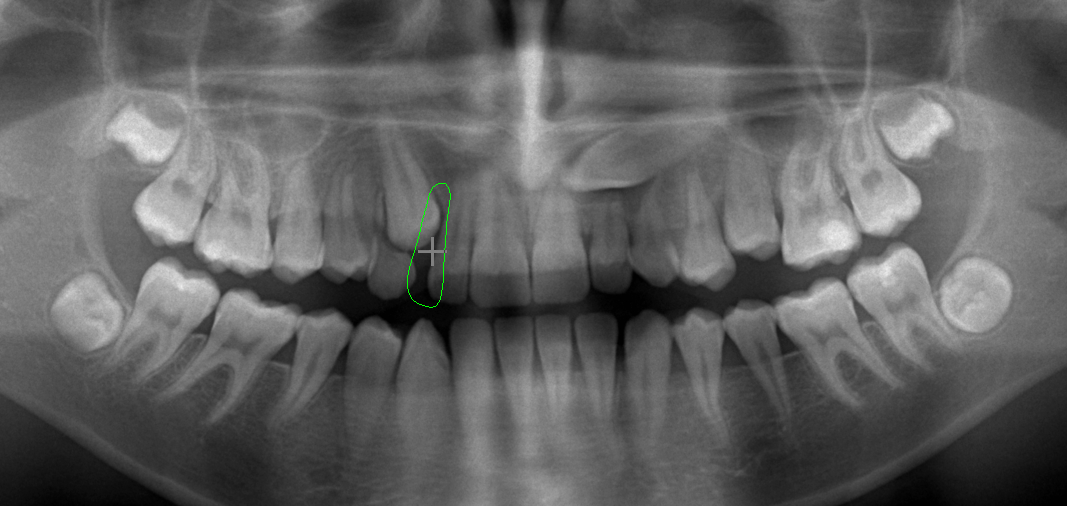
\includegraphics[width=\linewidth]{manual_init}
  \captionof{figure}{Manual initialization}
  \label{fig:manual}
\end{figure}
\newpage
\subsection{Automatic Initialization}
Our automatic initialization is a bit more complex. It consists of different steps, described (broadly) in algorithm \ref{algo:auto} below.
\newline
\begin{algorithm}[H]
\hspace{0.4mm} Find mean position of tooth over all test images.\\
\hspace{0.4mm} For each test image, create a template of the incisors as a whole.\\
\hspace{0.4mm} Crop the input image to the mean position, found in step 1.\\
\hspace{0.4mm} For each template, find the score of the template matching the cropped image from the previous step.\\
\hspace{0.4mm} For each template, find the best matching location in the cropped image.
Given the score,\linebreak
\hspace{0.4mm} (a) If the score is $\geq$ 99\%, break and used this score and this location.\linebreak
\hspace{0.4mm} (b) Else, register this score and location.\\
\hspace{0.4mm} For each score and location add score$*$location to the location we are going to return, such that we have a weighted average. If step (a) has occured, the location of only that template is returned and no weighted average is calculated.\\
\hspace{0.4mm} Take the landmarks associated with the templates and average them out using the scores obtained from the previous step. If step (a) was followed, it will use one set of landmarks.\\
\hspace{0.4mm} Return the necessary landmark.
\caption{Automatic initialization}
\label{algo:auto}
\end{algorithm}
\vspace*{3mm}
\noindent We will now go deeper into the steps described in algorithm \ref{algo:auto}. We want to find an initial position to place the model we want to fit on the radiograph. To achieve the optimal position, we perform a number of steps. Firstly, all training landmarks are loaded and a minimal fitting bounding box is calculated, such that we have a bounding box over all test images in which all teeth are located. \\
\newline
Next, we load all the test images and we crop the image to the bounding box created from the landmarks associated with this image. The resulting image thus contains all the 8 incisors for the image.\\
\newline
Now we load the image of the person we are trying to fit which we crop to the global bounding box, calculated in the first step, assuming that in this new image the teeth are distributed in a similar fashion as in the training images. We now have a number of templates and the input image all cut out (as adequately as possible) to only have the incisors in the image.\\
\newline
In this next step we use OpenCV's \texttt{matchTemplate}\footnote{\url{http://docs.opencv.org/2.4/modules/imgproc/doc/object_detection.html}}. This method will take the templates created and slides them over the image that you want to match. In our case the teeth templates are matched against the input image. It returns, amongst others, the matching score (as a percentage) and the `best matching location' as an offset compared to the image over which you are sliding.\\
\newline
Next, we evaluate the scores and location that were obtained before. Firstly, if the method finds a score that is greater than or equal to 99\%, this location and score will be used solely, without considering the rest. Otherwise, all scores and locations are registered. We calculate an average location by calculating the weighted average of all the locations found when matching the template using the associated scores as the weights. We now obtain an average location of where the teeth in this image are located. \\
\newline
Lastly, we take all the landmarks associated with the templates we used before and translate them such that they match the location/offset calculated in the previous step. Again, if there was a template with a match greater than 99\%, we only use this landmark. If not, we average the landmarks, again, using the scores from before, such that we obtain a set of average landmarks of all the teeth for this image. We now return the landmark of the tooth we have to initialize.\\
\newline
Below you can see the automatic initialization for two example images, which are not in the training data.
\begin{figure}[H]
\centering
\begin{minipage}{.5\textwidth}
  \centering
  \captionsetup{justification=centering}
  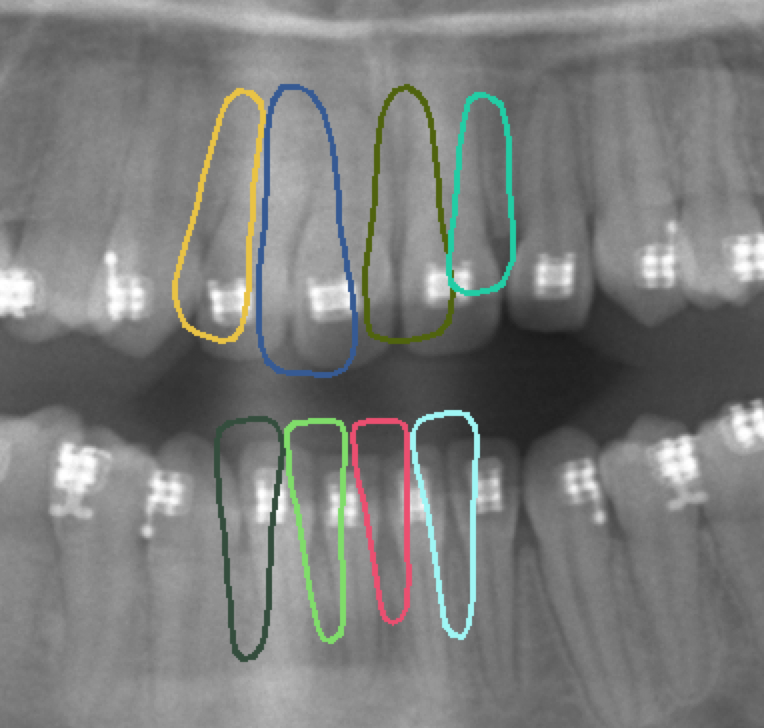
\includegraphics[width=\linewidth]{auto1}
  \captionof{figure}{Automatic initialization for person 27}
  \label{fig:auto1}
\end{minipage}%
\hspace*{4Mm}
\begin{minipage}{.5\textwidth}
  \centering
  \captionsetup{justification=centering}
  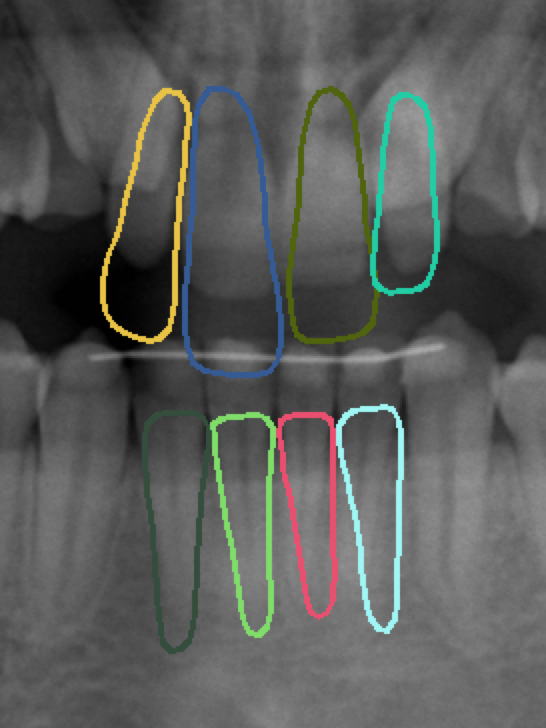
\includegraphics[width=\linewidth]{auto2}
  \captionof{figure}{Automatic initialization for person 17}
  \label{fig:auto2}
\end{minipage}
\end{figure}
For the teeth in figure \ref{fig:auto1}, this method works adequately, however this is not the case in figure \ref{fig:auto2}. This is due to the fact that this radiograph is slightly different from the `average radiograph': the teeth are positioned a bit higher.
In hindsight, we realise that this approach is not the most optimal one. In general: if we present a radiograph which has different proportions or where the teeth are aligned in a very different manner, this initialization behaves poorly. 

\subsection{Fitting procedure}

\subsubsection{Strongest Edge}\label{sec:stredge}

As proposed in \cite{cootes2000introduction}, we could fit the model to a new image by moving the initial points to the strongest edge in their surrounding. To find this edge, we consider a region of k pixels along the normal on the curve defined by the landmarks. The position with the strongest edge is then selected as the next position for the landmark point.

~\\This method has its flaws, since the real edge of a tooth is not necessarily the strongest edge present. Neighbouring teeth may have stronger edges, causing the model to be malformed. Another problem occurs when fitting the root of a tooth. The roots are less clearly delineated and therefore harder to fit to.

\subsubsection{Grey Level Models}\label{glms}

Another method proposed in \cite{cootes2000introduction} is to include local grey level information into the fitting procedure. For each landmark, a profile of the grey levels of a region along the normal is created. When fitting, a similar profile is extracted and matched with the ground truth profiles. The point with the best match is then selected as the next point to move towards.

\section{Evaluation of the Results}

\subsection{Examples of Manual Segmentation}

Figure \ref{fig:method1man} shows the result (in blue) of the segmentation when using the strongest edge method and with manual initialisation. Figure \ref{fig:method2man} shows the result (in blue) of the segmentation when using the grey level models and manual initialisation. Both figures are from radiograph 03. The green shapes show the ground truth for each tooth.

\begin{figure}[H]
\centering
\begin{minipage}{.4\textwidth}
  \centering
  \captionsetup{justification=centering}
  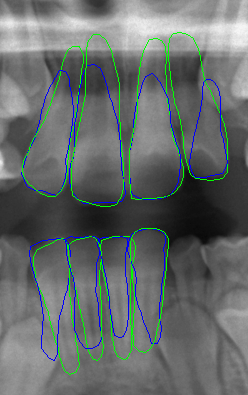
\includegraphics[width=\linewidth]{03_method1_manual}
  \captionof{figure}{Segmentation with manual initialisation and strongest edge fitting}
  \label{fig:method1man}
\end{minipage}%
\hspace*{4Mm}
\begin{minipage}{.4\textwidth}
  \centering
  \captionsetup{justification=centering}
  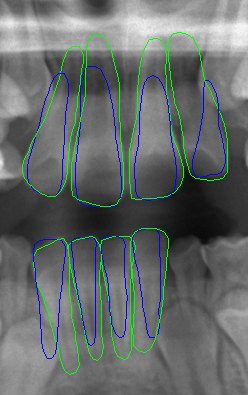
\includegraphics[width=\linewidth]{03_method2_manual}
  \captionof{figure}{Segmentation with manual initialisation and grey level model fitting}
  \label{fig:method2man}
\end{minipage}
\end{figure}

\subsection{Examples of Automatic Segmentation}

Figure \ref{fig:method1auto} shows the result (in blue) of the segmentation when using the strongest edge method and with automatic initialisation. Figure \ref{fig:method2auto} shows the result (in blue) of the segmentation when using the grey level models and automatic initialisation. Both figures are from radiograph 02. The green shapes show the ground truth for each tooth.

\begin{figure}[H]
\centering
\begin{minipage}{.4\textwidth}
  \centering
  \captionsetup{justification=centering}
  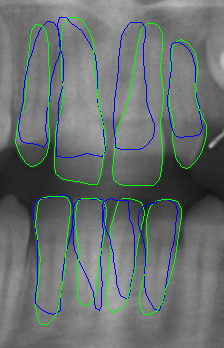
\includegraphics[width=\linewidth]{02_method1_auto}
  \captionof{figure}{Segmentation with automatic initialisation and strongest edge fitting}
  \label{fig:method1auto}
\end{minipage}%
\hspace*{4Mm}
\begin{minipage}{.4\textwidth}
  \centering
  \captionsetup{justification=centering}
  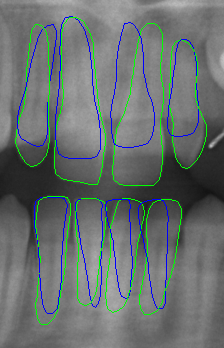
\includegraphics[width=\linewidth]{02_method2_auto}
  \captionof{figure}{Segmentation with automatic initialisation and grey level model fitting}
  \label{fig:method2auto}
\end{minipage}
\end{figure}

\subsection{Fitting Procedure Evaluation}

As mentioned in section \ref{sec:stredge}, fitting a model to a new image using the strongest edge has some drawbacks. To combat this issue, we tried to implement the grey level model technique as described in section \ref{glms}. However, this method did not produce great results. In most cases the shape would shrink or expand out of control. For this reason, the strongest edge method - while being a poor fitting method - still performed better than the grey level model method. Possible explanations for this poor performance might be a bad implementation of the method, or a badly chosen stop condition (the stop condition used to indicate whether or not convergence has occured.)

\section{Discussion}

\subsection{Preprocessing Alternatives}

A number of different filtering techniques could be applied to the radiographs in order to reduce noise and enhance the images. For example, the Radiographic Impulsive Noise removal filter proposed by Iuri Frosio (\cite{rainfilter}) could be applied. Other filters such as a bilateral filter or different histogram equalization methods could also be applied, depending on the desired result. For our application, the currently used filters sufficed.

\subsection{Automatic Initialization Alternatives}

Our approach for automatic initialization behaves poorly when the radiograph presented is different from the radiographs in the training set. In our initialization we try to match the template for the 8 incisors as a whole. In this regard we should have opted to match each teeth separately or, perhaps even better, separately for the upper and lower jaw. An alternative to using the template matching method provided by OpenCV, we could have tried to use a more general approach using PCA. \\~\\
Another possibility could have been to create a detection algorithm, such as the face detection algorithm, and use that for detecting teeth in a bounded area of a picture. This would only be possible if we had a larger set of teeth to our disposal. In the same manner we could have opted to create a (deep) learning algorithm to detect teeth in an image.

\subsection{General Discussion}
Overall, we feel like the solution we came up with performs well. Of course, using manual initialization this makes sense: you practically `tell' the program where to search for the teeth. In hindsight, our automatic initialization might have been constructed using an approach that is too brute force or `hacky', if you will. To conclude: we are positive about our approach and along the way we have learned a lot of new techniques and approaches regarding detection algorithms and computer vision.

\newpage
\addcontentsline{toc}{section}{References}

\bibliographystyle{apalike}
\bibliography{ref}

\end{document}
